% ============================================================
% DIAGRAM: CNN / LeNet-5 Architecture (1989/1998)
% ============================================================
% Caption: Figure 4.1: LeNet-5 CNN architecture.
%          (Adapted from LeCun et al., 1998, p. 2280)
% ============================================================

\documentclass[tikz,border=10pt]{standalone}
\usepackage{tikz}
\usepackage{amsmath}
\usepackage{amsfonts}

\usetikzlibrary{shapes,arrows,positioning,fit,calc,backgrounds}

\begin{document}

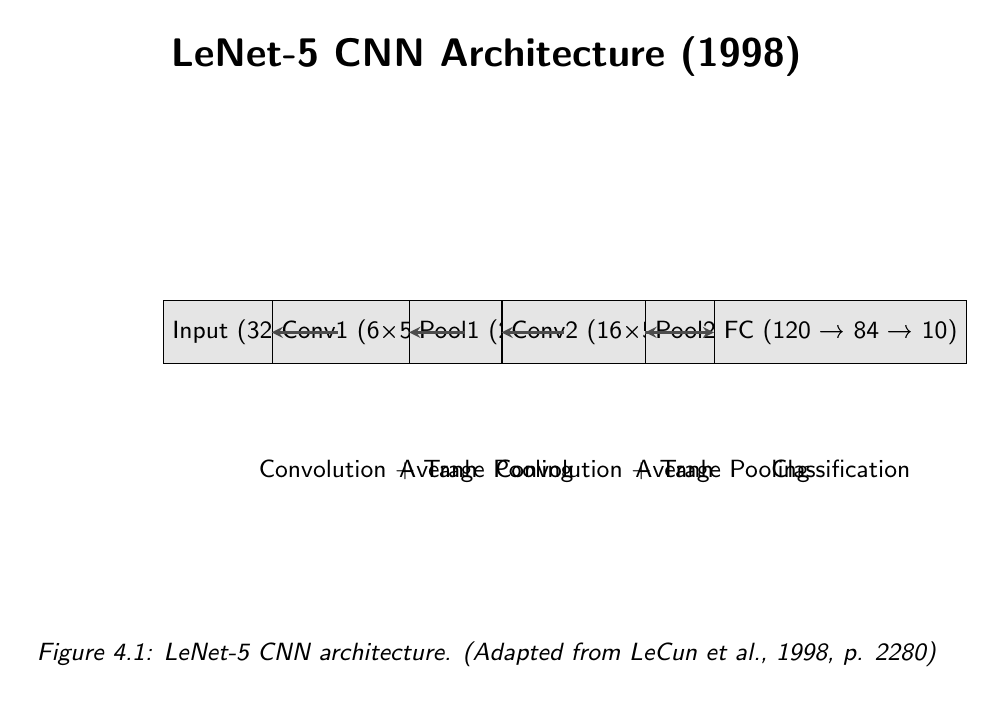
\begin{tikzpicture}[
    layer/.style={draw, rectangle, minimum width=1.2cm, minimum height=0.8cm, fill=gray!20, font=\sffamily\small},
    edge/.style={-stealth, thick, draw=black!70},
    label/.style={font=\sffamily\small},
    title/.style={font=\sffamily\Large\bfseries},
    caption/.style={font=\sffamily\small\itshape},
]

\node[title] at (0, 3.5) {LeNet-5 CNN Architecture (1998)};

% Layers
\node[layer] (input) at (-3, 0) {Input (32×32)};
\node[layer] (conv1) at (-1.5, 0) {Conv1 (6×5×5)};
\node[layer] (pool1) at (0, 0) {Pool1 (2×2)};
\node[layer] (conv2) at (1.5, 0) {Conv2 (16×5×5)};
\node[layer] (pool2) at (3, 0) {Pool2 (2×2)};
\node[layer] (fc) at (4.5, 0) {FC (120 → 84 → 10)};

\draw[edge] (input) -- (conv1);
\draw[edge] (conv1) -- (pool1);
\draw[edge] (pool1) -- (conv2);
\draw[edge] (conv2) -- (pool2);
\draw[edge] (pool2) -- (fc);

% Labels
\node[align=center, font=\sffamily\small, anchor=north] at (-1.5, -1.5) {Convolution + Tanh};
\node[align=center, font=\sffamily\small, anchor=north] at (0, -1.5) {Average Pooling};
\node[align=center, font=\sffamily\small, anchor=north] at (1.5, -1.5) {Convolution + Tanh};
\node[align=center, font=\sffamily\small, anchor=north] at (3, -1.5) {Average Pooling};
\node[align=center, font=\sffamily\small, anchor=north] at (4.5, -1.5) {Classification};

\node[caption, anchor=north] at (0, -3.8) {
  Figure 4.1: LeNet-5 CNN architecture. (Adapted from LeCun et al., 1998, p. 2280)
};

\end{tikzpicture}
\end{document}
